  % This is "sig-alternate.tex" V2.0 May 2012
% This file should be compiled with V2.5 of "sig-alternate.cls" May 2012
%
% This example file demonstrates the use of the 'sig-alternate.cls'
% V2.5 LaTeX2e document class file. It is for those submitting
% articles to ACM Conference Proceedings WHO DO NOT WISH TO
% STRICTLY ADHERE TO THE SIGS (PUBS-BOARD-ENDORSED) STYLE.
% The 'sig-alternate.cls' file will produce a similar-looking,
% albeit, 'tighter' paper resulting in, invariably, fewer pages.
%
% ----------------------------------------------------------------------------------------------------------------
% This .tex file (and associated .cls V2.5) produces:
%       1) The Permission Statement
%       2) The Conference (location) Info information
%       3) The Copyright Line with ACM data
%       4) NO page numbers
%
% as against the acm_proc_article-sp.cls file which
% DOES NOT produce 1) thru' 3) above.
%
% Using 'sig-alternate.cls' you have control, however, from within
% the source .tex file, over both the CopyrightYear
% (defaulted to 200X) and the ACM Copyright Data
% (defaulted to X-XXXXX-XX-X/XX/XX).
% e.g.
% \CopyrightYear{2007} will cause 2007 to appear in the copyright line.
% \crdata{0-12345-67-8/90/12} will cause 0-12345-67-8/90/12 to appear in the copyright line.
%
% ---------------------------------------------------------------------------------------------------------------
% This .tex source is an example which *does* use
% the .bib file (from which the .bbl file % is produced).
% REMEMBER HOWEVER: After having produced the .bbl file,
% and prior to final submission, you *NEED* to 'insert'
% your .bbl file into your source .tex file so as to provide
% ONE 'self-contained' source file.
%
% ================= IF YOU HAVE QUESTIONS =======================
% Questions regarding the SIGS styles, SIGS policies and
% procedures, Conferences etc. should be sent to
% Adrienne Griscti (griscti@acm.org)
%
% Technical questions _only_ to
% Gerald Murray (murray@hq.acm.org)
% ===============================================================
%
% For tracking purposes - this is V2.0 - May 2012

\documentclass{sig-alternate}
\usepackage{pygmentize}
\usepackage{minted}
\usepackage{graphicx}
\usepackage{xcolor,listings}
\usepackage{textcomp}
\lstset{upquote=true}

\begin{document}
%
% --- Author Metadata here ---
\conferenceinfo{Data For Good Exchange, 2015}\\

\title{Optimizing Local Smoke Alarm Inspections\\with Federal Data}
%
% You need the command \numberofauthors to handle the 'placement
% and alignment' of the authors beneath the title.
%
% For aesthetic reasons, we recommend 'three authors at a time'
% i.e. three 'name/affiliation blocks' be placed beneath the title.
%
% NOTE: You are NOT restricted in how many 'rows' of
% "name/affiliations" may appear. We just ask that you restrict
% the number of 'columns' to three.
%
% Because of the available 'opening page real-estate'
% we ask you to refrain from putting more than six authors
% (two rows with three columns) beneath the article title.
% More than six makes the first-page appear very cluttered indeed.
%
% Use the \alignauthor commands to handle the names
% and affiliations for an 'aesthetic maximum' of six authors.
% Add names, affiliations, addresses for
% the seventh etc. author(s) as the argument for the
% \additionalauthors command.
% These 'additional authors' will be output/set for you
% without further effort on your part as the last section in
% the body of your article BEFORE References or any Appendices.

\numberofauthors{3} %  in this sample file, there are a *total*
% of EIGHT authors. SIX appear on the 'first-page' (for formatting
% reasons) and the remaining two appear in the \additionalauthors section.
%
\author{
% You can go ahead and credit any number of authors here,
% e.g. one 'row of three' or two rows (consisting of one row of three
% and a second row of one, two or three).
%
% The command \alignauthor (no curly braces needed) should
% precede each author name, affiliation/snail-mail address and
% e-mail address. Additionally, tag each line of
% affiliation/address with \affaddr, and tag the
% e-mail address with \email.
%
\alignauthor
Marc DaCosta\\
       \affaddr{Co-founder, Enigma}\\
       \email{marc@enigma.io}
\alignauthor
Jeremy Krinsley\\
       \affaddr{Engineer, Enigma}\\
       \email{jak@enigma.io}
\alignauthor
Brian Abelson\\
       \affaddr{Engineer, Enigma}\\
       \email{brian@enigma.io}
}

\maketitle
\begin{abstract}
This paper outlines a fully-realized civic tool that predicts municipal blocks most likely to have homes without functioning smoke alarms and most likely to have residents who are at-risk for fire fatalities. Using a novel merge of the American Community Survey (ACS) and the American Housing Survey (AHS), we are able to model these two risk factors at the geography of census block groups, and with the aid of the TIGER Census dataset, return actual street addresses with associated risk scores. This tool represents a potential model for developing reusable civic analytic applications that can serve multiple cities while responding to local particularities.
\end{abstract}

\keywords{Civic Analytics, Fire Prevention, Census, ACS, AHS, TIGER }


\section{Intro}
We can expect 20,000 people to be injured or killed by fires in the United States this year. With over 130 million housing units across the country, 4.5 million of them do not have smoke detectors, placing their inhabitants at substantial risk. Driving this number down is the single most important factor for saving lives put at risk by fire.

A broad range of people are trying to address this problem, from local fire departments to the Red Cross. However, they all face the same problem: What doors do we knock on first?

A community knows best which blocks and which citizens are at risk for injury or death in a fire. First responders and outreach organizations know the facts of their municipality better than a dataset ever can: firemen know their districts; Red Cross volunteers and religious organizations know their local residents. These are the instincts that up to now have been the primary, if not the only resources available to identify at-risk homes and residents. 

With that in mind, we have gone farther than any previous effort to rank likelihood of smoke alarm risk by city block in the hopes that our work can offer more precise and granular leads for those who perhaps had no such prior resources. What we are able to present is a systematic ranking by city block for 209 cities that fall within 40 census-tabulated Metropolitan Statistical Areas (MSAs). We have furthermore developed a tool that allows these same first responders and active community members to improve the accuracy of local scores by uploading fire data via an API into our algorithm.

\section{Background}

In November of 2014 there was a house fire in the Broadmoor neighborhood of New Orleans that killed five people, including three children. The house did not have a smoke alarm in it. Enigma began working with New Orleans' Fire Department and Office of Performance and Accountability to develop a model that identified New Orleans blocks least likely to have residents with working smoke alarms, and most likely to experience a fire fatality. This enabled the New Orleans Fire Department to conduct a door-to-door outreach campaign to place smoke alarms in as many at-risk homes as possible. Drawing on learnings from New Orleans, we extended the model to apply to 178 municipalities within those census-defined Metropolitan Statistical Areas that contained the nation's 40 most populous cities, in hopes that more people can use and improve on our insights.


\section{Components}

The risk model and resulting tools were built off of a number of different federal census datasets. Below we outline these datasets and the ways in which we used them. We have also released all of the data components and algorithms that make this tool work, in hopes that others can improve upon what we have begun.

\subsection{AHS/ACS Merge}

The central crux of our work employs a systematic join of the American Housing Survey (AHS), a resource for nationally-representative, detailed housing characteristics, and the American Community Survey (ACS)\footnote{https://github.com/enigma-io/ahs-acs}, the census' most extensive and thorough demographic survey. This merge generates meaningful local data from a federal dataset that was once used only to describe characteristics normalized at the level of entire cities.

Making the ACS-AHS merge a machine-readable process greatly enhances the value of the data in the AHS, and by extension, enriches what we can learn about a given few blocks within the biggest metro-areas in the U.S. We are not the first\footnote{http://www.census.gov/content/dam/Census/programs-surveys/ahs/publications/CombiningAHS-ACS.pdf} to attempt a method for explaining the relationship between the two datasets. However, to the best of our knowledge, we have gone the furthest in making that process programmatic and fully machine-readable.

Many questions asked in the AHS directly mirror those asked in the ACS. For instance, both surveys ask about a respondent's age. While the ACS groups these responses into bucketed counts per block group (i.e. "Males under the age of 5" or "Females between the ages of 70 and 74"), the AHS simply records the respondent's actual age (4 or 72). While both surveys capture the same concept, they each record this information in different ways. Our merge enables translations between the two surveys by mapping these concepts into a common schema. This is useful as it allows models trained on AHS data to be scored on ACS data. 

We came up with these mappings by scanning the AHS Codebook for questions that were also asked in the ACS. For the most part, these were demographic variables and information about a respondent's household. In the case of the AHS, responses are recorded in categories (i.e. "married" = 3 and "divorce" = 4), or continuous numbers ("year house built" = 1964). On the other hand, as mentioned above, the ACS buckets responses by counts for census geographies, like block groups and tracts. In order to map the two surveys, we had to similarly bucket AHS responses into binary indicators. Here's an example of what this process looks like for "Marital Status":
\begin{minted}[
	frame=none,
	breaklines=true
]{yaml}
- concept: Marital Status 
  ahs:
        type: categorical
        var: hhmar 
        map:
            hhmar_married_spouse_present: 1
            hhmar_married_spouse_absent: 2
            hhmar_widowed: 3
            hhmar_divorced: 4
            hhmar_separated: 5
            hhmar_never_married:  6

  acs:
        table: B12001
        total: B12001001
        map:
            hhmar_married_spouse_present: [B12001005,B12001014]
            hhmar_married_spouse_absent: [B12001006, B12001015]
            hhmar_widowed: [B12001009, B12001018]
            hhmar_divorced: [B12001010, B12001019]
            hhmar_separated: [B12001007, B12001016]
            hhmar_never_married: [B12001003, B12001012]
\end{minted}

\subsection{Risk Model}

Armed with this novel dataset, we set about to develop a model to estimate the risk that residents of a particular census block group risk lack smoke alarms.  An outline of our approach is as follows:

\begin{enumerate} 
\item Leverage exploratory analysis to select an appropriate sample from the AHS.
\item Train a national-level Random Forest on the AHS.
\item Train one Random Forest for each MSA in the AHS with an added model weighting function.
\item Compute scores for the national and MSA-level models and merge.
\end{enumerate}

\subsubsection{Handling Missing Data in the AHS}

The AHS does not require that subjects respond to all questions. As a result, there's a lot of missing data. We deal with this problem via the following steps:

\begin{figure}
\centering 
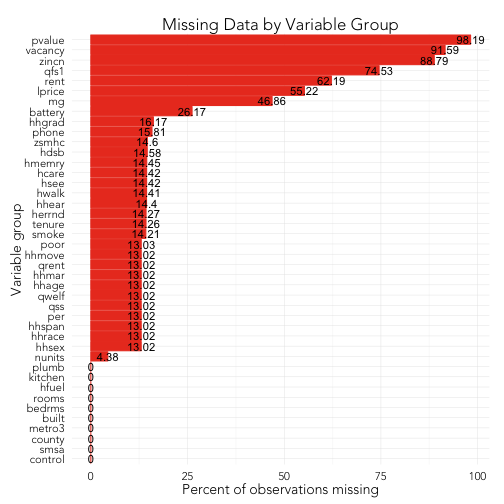
\includegraphics[scale=0.42]{missing-data-1.png}
\caption{Missing data in the AHS by variable group}
\end{figure}

\begin{enumerate} 
\item Drop all observations with greater than 90\% of missing variables. 
\item Drop all observations with a missing dependent variable.
\item Drop all variable groups with greater than 50\% of missing data (Figure 1).
\item Randomly impute missing data by sampling from it's existing distribution.
\end{enumerate}

Out of the 186,448 rows in the AHS, we were able to keep 155,108 through this process, or 83.2\% of the total. 

\subsubsection{Covariate Selection}

Through a simple correlation analysis, we settled on a number of variable groups in the AHS to use as covariates in our model:

\begin{itemize} 
\item ``built'' - The year the household was built. 
\item ``poor'' - Percentage of income relative to the poverty level. Observations with a missing dependent variable.
\item ``hhmove'' - The year the current resident moved in.
\item ``hhgrad'' - The education level of the homeowner.
\item ``hhrace'' - The race of the homeowner.
\item ``hhspan'' - Whether the homeowner is of Hispanic descent.
\item ``hfuel'' - The type of fuel the home uses for heating. 
\item ``tenure'' - The rental status of the homeowner.
\item ``mg'' - The mortgage status of the homeowner.
\end{itemize}

\begin{figure}
\centering 
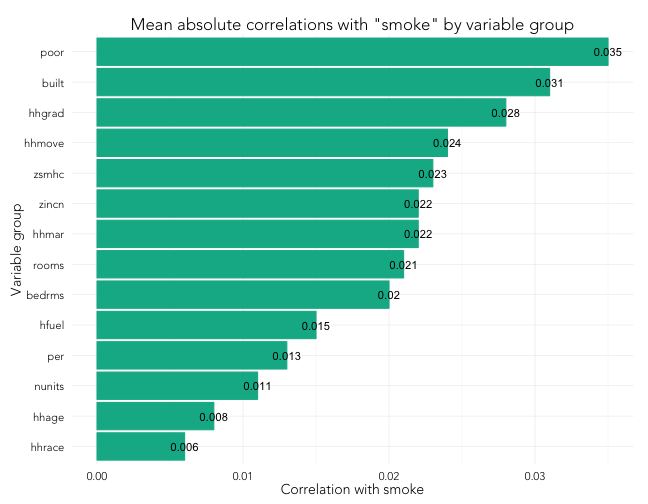
\includegraphics[scale=0.42]{explore-correlations-1-2.png}
\caption{Mean absolute correlations with "smoke" by variable group}
\end{figure}

These groups translated into the following formula (written in R syntax):

\begin{minted}[
	frame=none,
	breaklines=true
]{r}
# our model's formula
f <- smoke ~  
       built_1980_to_1989 +
       built_1960_to_1969 +
       built_2010_to_later +
       built_1990_to_1999 +
       built_1950_to_1959 +
       built_1939_or_earlier +
       poor_50_to_99 +
       poor_under_50  +
       poor_184_to_199 +
       poor_125_to_149 +
       poor_100_to_124 +
       poor_150_to_184 +
       hhmove_moved_in_1990_to_1999 +
       hhmove_moved_in_1969_or_earlier +
       hhmove_moved_in_2000_to_2009 +
       hhmove_moved_in_1970_to_1979 +
       hhmove_moved_in_1980_to_1989 +
       hhgrad_associates_degree +
       hhgrad_7th_or_8th_grade +
       hhgrad_9th_grade +
       hhgrad_doctorate_degree +
       hhgrad_5th_or_6th_grade +
       hhgrad_regular_high_school_grad +
       hhgrad_bachelors_degree +
       hhgrad_1st_2nd_3rd_4th_grade +
       hhgrad_11th_grade +
       hhgrad_less_than_1st_grade  +
       hhgrad_12th_grade_no_diploma +
       hhrace_hawaiian_pac_isl_only +
       hhrace_asian_only +
       hhrace_other +
       hhrace_black_only +
       hhrace_native_am_only +
       hhrace_white_only +
       hhspan_yes +
       tenure_renter_occupied +
       hfuel_wood +
       mg_yes
\end{minted}

\subsubsection{National Model}

First, we estimate a national Random Forest with the above formula on the entirety of our AHS sample.

Only 4\% of respondents answered negatively to the question "Do you have a working smoke alarm?" For such rare events, it can be difficult to generate a classifier which is equally sensitive to negative and positive outcomes. If we simply guessed that every respondent lacked a smoke alarm, we would be correct in 96\% of cases. However, since our goal is to identify those at risk for not having a smoke alarm, we want to maximize our accuracy when predicting these rare events, even if it means a decrease in the overall accuracy of our model.  We deal with this issue by oversampling respondents without smoke alarms when training the Random Forest. The degree of oversampling is determined by training identical models with different weights, and plotting the error rates (Figure 3). 

\begin{figure}
\centering 
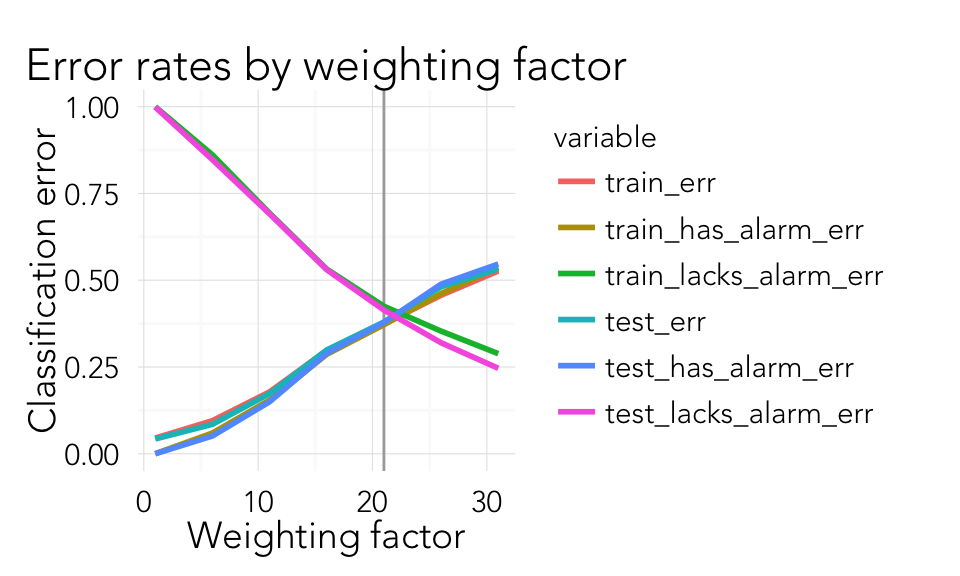
\includegraphics[scale=0.36]{test-rf-1.png}
\caption{Error rates by oversampling weight.}
\end{figure}

The national-level model suggests that, in general, race, poverty status, education level, and the date the householder moved in are strong predictors of a resident lacking a smoke alarm (Figure 4).  This model has an overall accuracy of 63\% and a true positive rate (the percentage of cases in which we accurately identify residents without smoke alarms) of 59\%.

\begin{figure}
\centering 
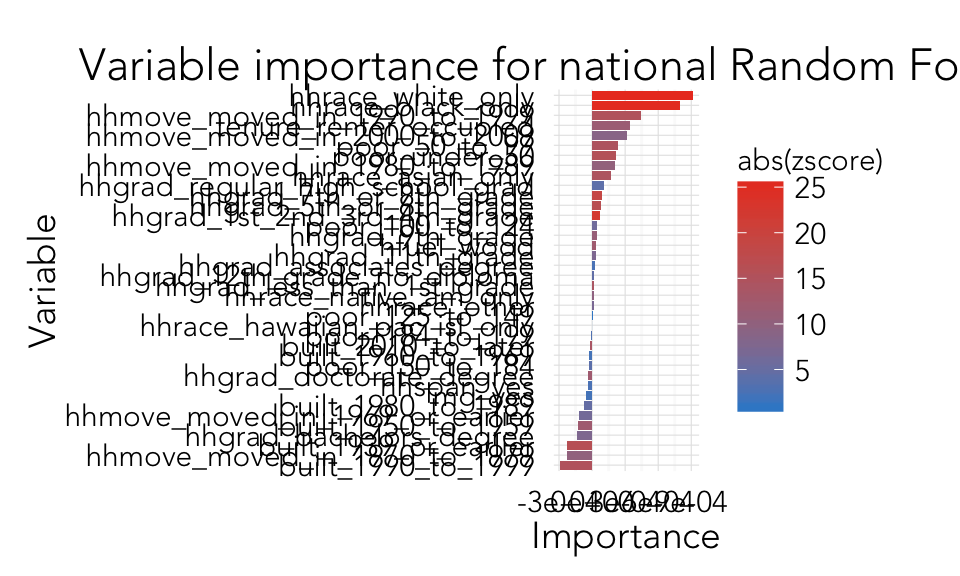
\includegraphics[scale=0.36]{var-importance-1.png}
\caption{Variable importance for national-level Random Forest.}
\end{figure}

\subsubsection{MSA Models}
We estimate MSA-level effects by training identical models for each MSA represented in the AHS. To select an appropriate list of MSAs to model, we explored the total number of respondents and respondents without smoke alarms per MSA (Figures 5 \& 6). We chose to eliminate all MSAs that have less than 2,000 total respondents.  This resulted in a list of 29 MSAs out of a possible 147. It should be noted here that while we ran our analysis on only 29 MSAs, we extrapolated normalized nation-wide scores to 41 MSAs.

\begin{figure}
\centering 
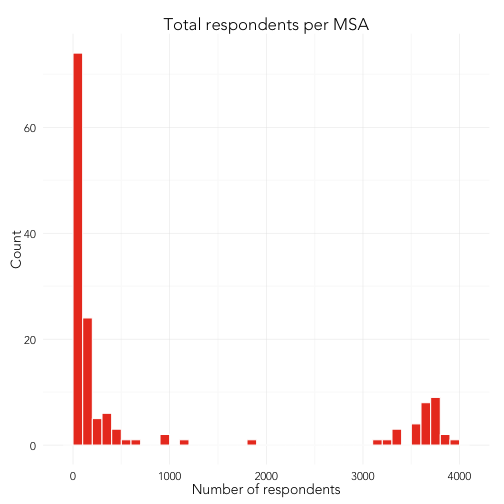
\includegraphics[scale=0.42]{compute-msa-stats-histogram-1.png}
\caption{Total respondents per MSA.}
\end{figure}

\begin{figure}
\centering 
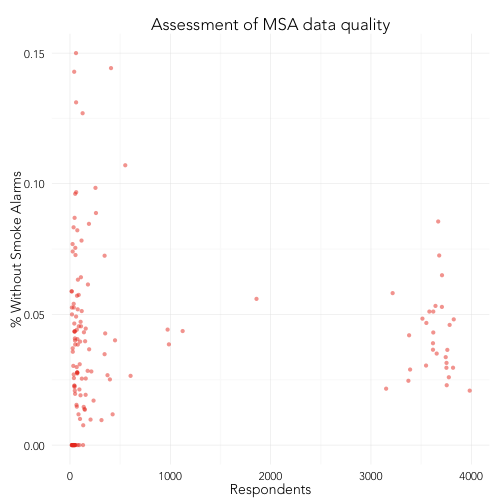
\includegraphics[scale=0.42]{compute-msa-stats-scatter-1.png}
\caption{Total respondents per MSA by percent without smoke alarms.}
\end{figure}

We also adjusted the oversampling weight for each MSA-level model by the percentage of respondents without smoke alarms. Initial tests demonstrated that this metric was highly correlated with the false positive rate (Figure 7). This process effectively normalizes the overall error rate of MSA-level models regardless of sample size (Figure 8).  On average, the MSA models have an overall accuracy of 61\% and a true positive rate of 55\%. 

\begin{figure}
\centering 
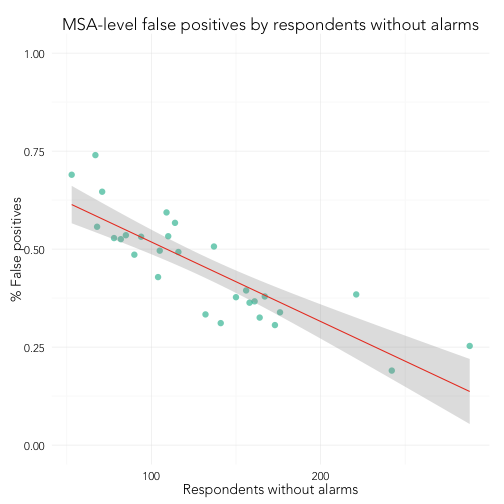
\includegraphics[scale=0.42]{rf-msas-metrics-1.png}
\caption{False positives by respondents without smoke alarms per MSA.}
\end{figure}

\begin{figure}
\centering 
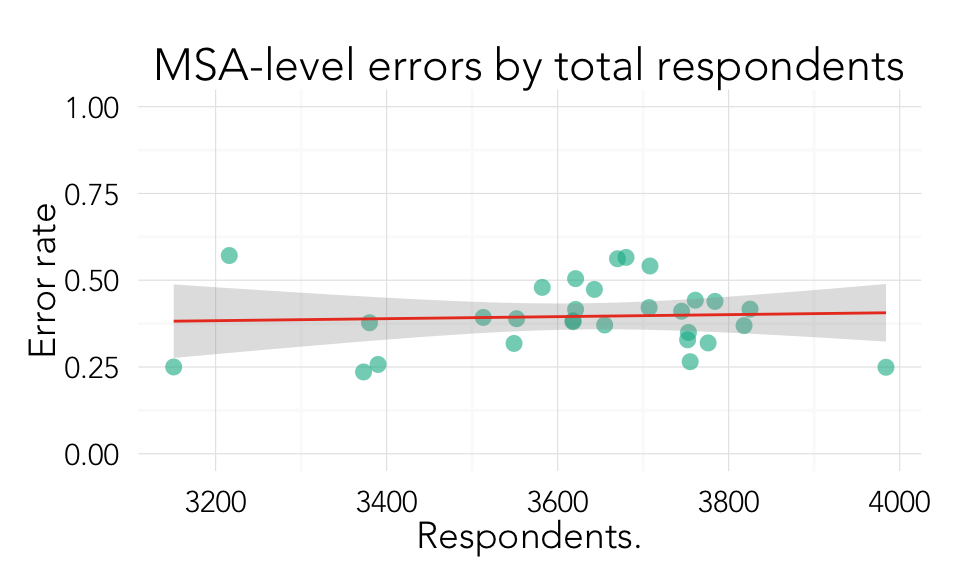
\includegraphics[scale=0.42]{rf-msas-metrics-3.png}
\caption{Overall error by total respondents per MSA.}
\end{figure}

\subsubsection{Computing Risk Scores}

Risk scores are computed by applying the models trained on the AHS to census block group-level data from the ACS. These scores represent the probability that residents in a given block group lack smoke alarms. In the case a block group falls within our list of selected MSAs, we average its national score with it's MSA-specific score. In this manner, we aim to capture national and local-level variations in the factors associated with smoke alarm risk (Figures 9 \& 10). A more sophisticated approach might employ a single multilevel model rather than an ensemble of a national and MSA-level model. Interestingly, there did not appear to be a strong relationship between national and MSA-level risk scores (Figure 11).  Without a present means of verifying the validity of these scores, we cannot be certain whether this is product of the model's relatively high error rate, local variations, or some combination thereof.

\begin{figure}
\centering 
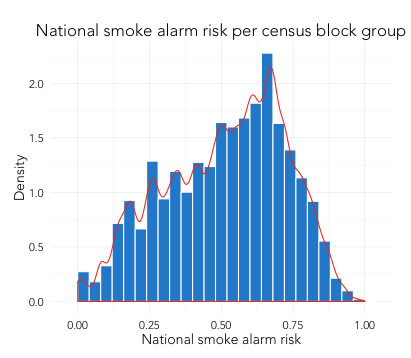
\includegraphics[scale=0.42]{score-metrics-1.png}
\caption{Distribution of overall risk score per census block group.}}
\end{figure}

\begin{figure}
\centering 
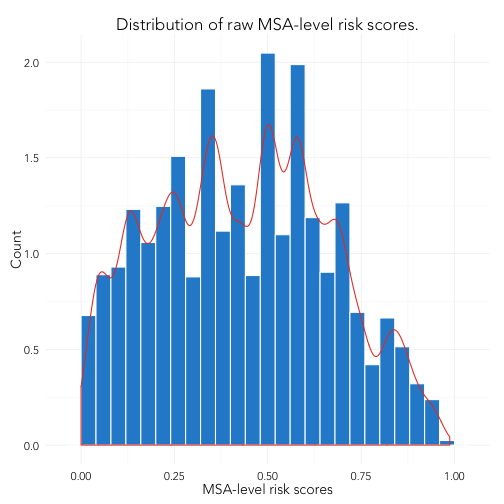
\includegraphics[scale=0.42]{score-metrics-2.png}
\caption{Distribution of MSA-level risk score per census block group.}}
\end{figure}

\begin{figure}
\centering 
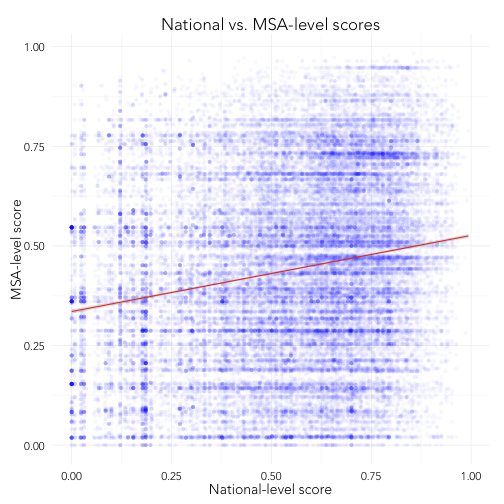
\includegraphics[scale=0.42]{score-metrics-3.png}
\caption{Relationship of national and MSA-level scores.}}
\end{figure}

\subsection{TIGER Geocoder}

The Census Bureau maintains a comprehensive and deeply granular dataset of geographical features for the United States. The Topologically Integrated Geographic Encoding and Referencing (TIGER) dataset contains ESRI shapefiles that describe boundaries from the state level down to census blocks, and includes a diverse collection of geographies in between, from congressional districts to tribal reservations. By loading these files into a database capable of spatial queries, we gain the ability to situate the results of our risk model in specific areas of cities, and even on specific street blocks.

We used the Census TIGER dataset in conjunction with the PostGIS TIGER geocoder extension for the PostgreSQL database. It should be noted that our entire stack is fully open source and free to reproduce. To that end, we built a package that makes it easy for civic coders with basic skills to spin up the spatial tools that we employed for this project.\footnote{https://github.com/enigma-io/ansible-tiger-geocoder-playbook} 

\subsubsection{Block Group Geographic Join}

We first relied on the TIGER dataset to map our risk scores to specific geographical boundaries within the cities we analyzed. Each record in the ACS maps to a census block group, an area that can range in population from 600 to 3,000 citizens, and which is considered the smallest geographical entity deemed to still present valid sample data. This means that census block groups are highly variable in area. In a place like New York City, a census block group will consist of only a few blocks, whereas some areas of Alaska contain block groups that are thousands of square miles.

Of the total 220,740 block groups in the U.S., we generated relevant scores for those with a population density over RATIO that fell within one of the 29 we deemed data-rich enough to provide reliable scores.

Finding the relevant block groups using these aforementioned tools is relatively trivial. For instance, to find block group ids that are in any given MSA, the query looks like:

\begin{lstlisting} [
           language=SQL,
           showspaces=false,
           basicstyle=\ttfamily,
           numbers=left,
           numberstyle=\tiny,
           commentstyle=\color{gray},
           breaklines=true
        ]
SELECT 
  bg_id as block_group_id
FROM 
  -- the block groups TIGER table
  tiger.bg, 
  -- the MSAs TIGER table
  -- for metro and micro areas
  tiger.cbsa
WHERE 
  -- the lsad field is 'M1' for metro 
  -- and 'M2' for micro
  tiger.cbsa.lsad='M1'
AND
  ST_Intersects(
    tiger.bg.the_geom,
    tiger.cbsa.the_geom
   )
\end{lstlisting}

\subsubsection{Address Range Resolution}

We also used the TIGER data to create a master CSV of all street blocks that fell within geographies we analyzed, coupled with their risk scores.

The TIGER data collection includes a comprehensive address ranges table that defines every street, by block, in the U.S. The 2.9m row table includes the name of a street and its left and right-side address ranges. Using geospatial querying in PostGIS, we grouped these address ranges by census block groups, and thereby joined every city block and address range to the relevant census block score in our model. 

The method employed for this was simple: for each street in the address features table, shift the line-segment defined as that street's geographical location a few meters to the left, and then a few to the right, and join these off-based line-segments to the census block geographies within which they fall. This small geographical transform for each street reduced the ambiguities that arise when streets form the border between two census block groups. In those cases, addresses on side A of a street ought to be associated with census block group A, and addresses on side B ought to be associated with census block group B. Without enacting this small transform, addresses will associate with both block groups they border, rather than the one they are actually within.

The query ultimately joins the two shifted street sides:

\begin{lstlisting} [
           language=SQL,
           showspaces=false,
           basicstyle=\ttfamily,
           numbers=left,
           numberstyle=\tiny,
           commentstyle=\color{gray},
           breaklines=true
        ]
with right_side as (
    SELECT distinct
        block_group.bg_id as block_group_id,
        right_side.fullname as street_name,
        right_side.lfromhn as from_addr,
        right_side.ltohn as to_addr
    FROM
        tiger.addrfeat as right_side,
        tiger.bg as block_group
    WHERE ST_Intersects(block_group.the_geom, right_side.the_geom)
    -- intersections of 0 length occur!
    AND St_Length(ST_Intersection(block_group.the_geom, right_side.the_geom)) > 0
    AND ST_Intersects(
        -- offset the street by a small margin
        ST_OffsetCurve(ST_LineMerge(right_side.the_geom), .00001),
        block_group.the_geom
    )
),

-- identical to right_side, with offset curve set negative
left_side as (
    SELECT distinct
        block_group.bg_id as block_group_id,
        left_side.fullname as street_name,
        left_side.lfromhn as from_addr,
        left_side.ltohn as to_addr
    FROM
        tiger.addrfeat as left_side,
        tiger.bg as block_group
    WHERE ST_Intersects(block_group.the_geom, left_side.the_geom)
    -- intersections of 0 length occur!
    AND St_Length(ST_Intersection(block_group.the_geom, left_side.the_geom)) > 0
    AND ST_Intersects(
        -- offset the street by a small margin
        ST_OffsetCurve(ST_LineMerge(left_side.the_geom), -.00001),
        block_group.the_geom
    )
)

SELECT * FROM right_side
UNION ALL
SELECT * FROM left_side
\end{lstlisting}

This query fails to return distinct results when streets are simultaneously extremely curvy and very close to each other. There are a low number occurrences of this anomaly. Out of 14,677,020 distinct listed street ranges, 99.51\% fall within a single block group, .49\% fall within two, and only 103 blocks fall within three. Clearly there is space here to refine our work, but for practical applications, the duplication of streets within block groups are not significant enough to truly hamper outreach work on the ground.

\section{Civic Tools}

The primary purpose of this project was not analysis and research, but rather a suite of open-sourced tools that make decision-making easier for fire departments and organizations involved in fire risk mitigation. Here we outline the primary output of our efforts to date.

\subsection{Smoke Risk Portal}

All of the tools outlined below are hosted on our site, which is designed to engage directly with those who are most likely to use them. 

\subsection{Interactive Map}

We designed a granular map for every geography we analyzed so that those involved in outreach can quickly assess the risk scores for their particular locality. The map depicts census block groups for each of the 41 MSAs for which our model applies, shaded to reflect relative likelihood that an area contains households that do not have a smoke alarm.

\subsection{Address/Score CSV}

While the map offers an immediate bird's eye view of the model, we offer risk scores by address ranges as a downloadable CSV.

These CSVs are the result of joining the geospatial analysis above with our model. Each record in the CSV lists a street name, street ``start'' address and ``end'' address, a risk score, and the state and county within which the block is located, along with details about the block group associated with the street.

These CSVs were built with the intention that they would provide maximum value to local first responder and outreach communities. The data model was designed so that someone with the basic ability to order an Excel spreadsheet could quickly organize a list of the highest risk blocks by street name and address range for their local districts and areas of interest.

\subsection{Data Augmentation API}
While our model is built entirely from federal data, our initial work with the city of New Orleans also factored in local fire incident data. In that spirit, we built an analysis API that further enhances our risk scores when local fire incident is uploaded to an endpoint. The API accepts a CSV of local fire incident data, which must include:
\begin{itemize}
\item a latitude column (``latitude'')
\item a longitude column (``longitude'')
\item each row must represent a fire incident
\end{itemize}

It should be noted that our analysis pipeline disregards any additional features in the CSV beyond these simple requirements, thereby reducing the amount of data munging required to generate enhanced scores.

Given this information, we compute an indicator of fire incidents per census block group normalized for the included area. We also include a similar indicator which captures to percentage of "at-risk" populations (\% of people aged less than 5 or greater than 65). We then average these indicators of fire risk and at-risk population with the overall risk for residents not having smoke alarms.  This score represents our best attempt to preference populations simultaneously at risk for lacking smoke alarms and dying in home fires.

\section{Conclusion}

Prioritizing outreach efforts for fire prevention can be difficult without knowing which doors to knock on. By drawing together multiple public data sets, we have developed a predictive model and analysis pipeline that increases the likelihood of finding at-risk populations.

Our goal is to provide a tool that helps fire departments and other groups work more efficiently. Local fire department outreach coordinators can combine their internal databases about local fires with geographically granular profiles for smoke alarm risk. 

This is only a first step. The City of New Orleans will soon release its first round of results following an initial pilot of this data-driven outreach program. That will provide valuable insight into ways that our model can be improved since we currently rely on federal data without the assistance of a reliable training set to verify results. 

\section{Acknowledgements}
Throughout this project, we were in close collaboration with representatives of the Red Cross and DataKind.

\end{document}
